% !TEX root = _main.tex

\begin{figure*}[tb]
	\centering
	\begin{minipage}{0.36\hsize}
		\centering
		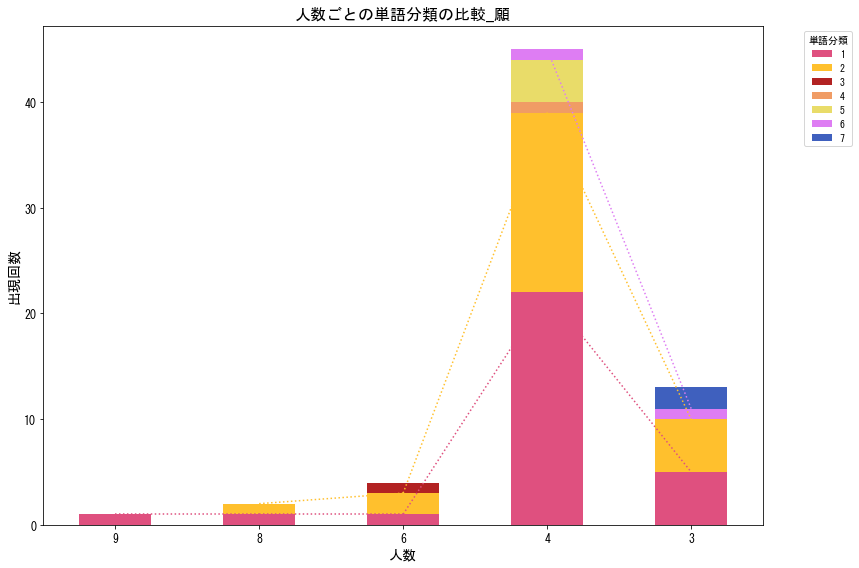
\includegraphics[width=\hsize]{fig/negau-ninzu.png}
		\caption{「願」人数時代別使用意味比較}
		\label{fig:negau-ninzu}
	\end{minipage}
	\begin{minipage}{0.62\hsize}
		\centering
		\captionof{table}{「願」人数別時代ごとの\kyokusu （()内は割合）}
		\label{tab:negau-uchi}
		\begin{tabular}{c|cccccc}
			\hline
			「願」の分類  & ９人時代      & ８人時代     & ６人時代     & ４人時代      & ３人時代     & 合計        \\
			\hline\hline
			1:未来，希望 & 1 (100.0) & 1 (50.0) & 1 (25.0) & 22 (48.9) & 5 (38.5) & 30 (46.2) \\
			2:恋，恋愛  & 0 (0.0)   & 1 (50.0) & 2 (50.0) & 17 (37.8) & 5 (38.5) & 25 (38.5) \\
			3:過去    & 0 (0.0)   & 0 (0.0)  & 1 (25.0) & 0 (0.0)   & 0 (0.0)  & 1 (1.5)   \\
			4:相手に願う & 0 (0.0)   & 0 (0.0)  & 0 (0.0)  & 1 (2.2)   & 0  (0.0) & 1 (1.5)   \\
			5:勝利    & 0 (0.0)   & 0 (0.0)  & 0 (0.0)  & 4 (8.9)   & 0 (0.0)  & 4 (6.2)   \\
			6:愛     & 0 (0.0)   & 0 (0.0)  & 0 (0.0)  & 1 (2.2)   & 1 (7.7)  & 2 (3.1)   \\
			7:音楽    & 0 (0.0)   & 0 (0.0)  & 0 (0.0)  & 0 (0.0)   & 2 (15.4) & 2 (3.1)   \\
			\hline
			合計      & 1         & 2        & 4        & 45        & 13       & 65        \\
			\hline
		\end{tabular}
	\end{minipage}
\end{figure*}
